
%%%%%%%%%%%%%%%%%%%%%%%%%%%%%%%%%%%%%%%%%%%%%%%%%%%%%%%%%%%%%%%%%%%%%%%%%
%           Capítulo 2: MARCO TEÓRICO - REVISIÓN DE LITERATURA
%%%%%%%%%%%%%%%%%%%%%%%%%%%%%%%%%%%%%%%%%%%%%%%%%%%%%%%%%%%%%%%%%%%%%%%%%

\chapter{Marco teórico}

\section{Calculo de capacidad de corriente en pistas de circuitos impresos}



Antes de comenzar con la fabricación de un diseño de PCBs se debe de considerar el tamaño de pistas necesarios para el manejo de corrientes para cada circuito desarrollado, por esa razón mediante un análisis empírico se debe avanzar en el diseño.\\

En la actualidad los requerimientos de corriente llevan al límite la capacidad de reducir el ancho de las pistas y espacios debido a que se desarrollan componentes cada vez más pequeños y sistemas igualmente más compactos, esto obliga al desarrollador a adaptarse a estos nuevos requerimientos.\\

Para encontrar una solución a esta eventualidad es necesario recurrir a estudios en estos temas que nos permita acercarnos al límite y para ello debemos de considerar todos los parámetros que influyan en nuestro sistema, obteniendo así resultados más precisos. En nuestro caso nos basaremos en los gráficos publicados en el IPC2152 ``Standard for Determining Current Carry Capacity in Printed Board Design'' en 2009, este estándar es ampliamente utilizado en muchos proyectos que requieran este tipo de análisis. \\

Para el correcto entendimiento de los procesos que influyen en las pistas por el paso de la corriente debemos de recordar que el paso de la corriente por un conductor produce en este una caída de potencial que esta gobernada por la ley de OHM (R=V/I), esta caída de potencial se disipa en forma de calor por el efecto Joule $Q=I^{2}Rt$. En nuestro el conductor es nuestra pista, su resistencia depende de varios factores, pero lo principal es su sección (ancho x espesor) y su longitud. El efecto térmico es en realidad el que nos interesa conocer al momento del dimensionamiento de la PCB. Por esta razón, para poder calcular una capacidad de transporte de corriente, hay que analizarlo en términos de incremento de temperatura. Fijando como un incremento maxico admisible.\\

Existen algunos parámetros que se deben de considerar importantes de conocer, ya que los mismos alteran o modifican el comportamiento termico de la pista, afectando de manera significativa, los mas importantes son:\\

\begin{itemize}
\item Corriente eléctrica que circula.
\item Tipo de material base.
\item Calculo de corriente de pistas.
\item Sección de la pista.
\item Espesor del laminado de cobre.
\item Espesor de la placa.
\item Presencia de planos de tierra o grandes áreas de cobre.
\item Ambiente de aplicación (gabinete, forzadores de aire, vacío, etc.)
\end{itemize}

Considerar todos estos parámetros en un modelo es bastante complicado, tanto que, en sí, el estándar fue fijado por medio de ensayos y presentando los resultados en forma de curvas. Mediante estos datos empíricos se hace una aproximación que se acerque al límite que deseamos, tomando en cuenta que es importante sobredimensionar dichos límites. \\

El cálculo que se realiza se basa en el fijado de una variación máxima de temperaturas admisibles. La variación térmica se define como un aumento de temperatura por encima de la temperatura inicial que experimenta el conductor. \\
Para el cálculo se requieren los gráficos ya antes mencionados que son dos. El primer grafico es una de las tres entradas y se trata de una serie de curvas que corresponden a los incrementos de temperatura desde diez a cien grados centígrados. En el eje de las ordenadas se grafica la corriente máxima en amperes y en el de las abscisas obtenemos la sección de la pista en milésimas de pulgada cuadrada. El segundo grafico tiene de igual manera tres entradas y en esta se centra en el espesor del cobre, adoptando los valores típicos en los que se fabrican las PCBs, llegando desde 0.5 hasta 3 Oz/ft2.\\

Los cálculos necesarios son sencillos y claros de realizar, para ello necesitaremos los siguientes datos:\\

\begin{itemize} 
\item Corriente máxima a soportar.
\item Incremento máximo de temperatura admisible.
\item Espesor de cobre del material utilizado.
\end{itemize}
Utilizando el valor de corriente nos ubicamos en el grafico 1 por el eje de las ordenadas y proyectamos el valor en forma paralela al eje de las abscisas hasta interceptar la curva que corresponde a la temperatura máxima admisible, luego tomamos el punto en las ordenadas hasta obtener el valor de las absisas que le corresponde. Ese valor es el valor de la sección cuadrada que debe de tener la pista.

\begin{figure}[H]
\centering
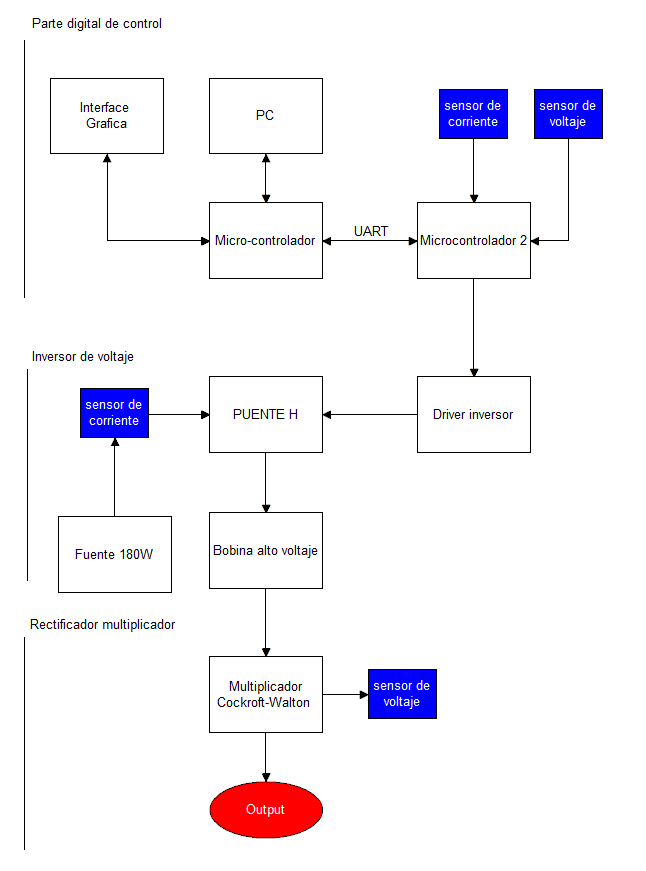
\includegraphics[width=12cm]{capitulo2/figs/figura1.png}
\caption{Calculo de ancho de pistas 1}
\end{figure}

\begin{figure}[H]
\centering
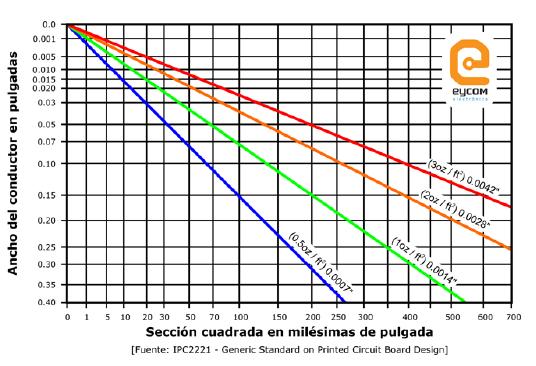
\includegraphics[width=12cm]{capitulo2/figs/figura2.png}
\caption{Calculo de ancho de pistas 1}
\end{figure}




\newpage
\section{Ruidos e interferencias}
\subsection{Ruidos en micro-controladores y sistemas digitales}

En particular no existe una forma tal cual para evitar ruidos en nuestros sistemas electrónicos, sino más bien dependiendo de las características de los proyectos se siguen distintos arreglos que mejoran la calidad de las señales que muchas veces, sin el trato adecuado pueden afectar a microcontroladores, PICs o distintos sistemas digitales o analógicos que se presenten. \\

Cuando diseñamos un circuito en general, es probable que funcione correctamente en un simulador o en el Protoboard, pero al momento de accionar o activar cargas de potencia o en señales de alta frecuencia los problemas de ruidos aparecen y las afectaciones pueden llegar a distorsionar una señal o causar estragos en nuestros componentes o cargas.\\

Debemos aclarar que los ruidos electrónicos, no afectan a todos los circuitos por igual, debemos de considerar el tipo de electrónica que estamos desarrollando, entre las que se encuentran circuitos de potencia, de alta frecuencia, componentes como microcontroladores, FPGAs, PICs, etc. que requieren estabilidad en alimentaciones o entradas. Considerando esto la eliminación de ruidos puede ser algo simple como condensadores cerámicos o electrolíticos, hasta la necesidad de realizar arreglos complicados.\\

En nuestro caso estaremos accionando transistores, MOSFETs, bobinas y componentes que requieren grandes consumos de corriente, es por ello que necesitamos tomar en cuenta ciertos aspectos para evitar que dicho ruido afecte al sistema en general o a componentes en específicos claves como el microcontrolador o el sistema de conexión al computador que se estará manejando.\\

Para resolver el problema con los ruidos electrónicos, debemos de actuar de forma pro-activa, es decir, tener en cuenta todos los detalles importantes de operación de nuestro circuito, antes de construirlo de forma definitiva. Para ello tenemos que tomar en cuenta que nuestro micro-controlador es un elemento digital y se deben de tomar todos los cuidados para un óptimo funcionamiento.\\

Teniendo en cuenta lo antes mencionado nos apegaremos a una lista de requerimientos que nuestro circuito deberá de cumplir para obtener el menor ruido posible. Nos concentraremos en esta primera lista en requerimientos necesarios para componentes digitales como micro-controladores.

\begin{itemize} 
\item Utilizar un condensador Bypass (0.1uF) entre los pines de alimentación y tierra del microcontrolador y de cada circuito integrado que componga al sistema.
\begin{figure}[H]
\centering
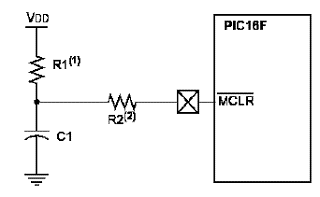
\includegraphics[width=8cm]{capitulo2/figs/fig3.png}
\caption{Condensador Bypass}
\end{figure}

\item Evitar dejar pines sin conexión. Llevarlos a GND, programando dichos pines como salidas y otorgándoles un valor de 0.

\item Utilizar condensadores de aterrizado del cristal.

\item Utilizar Reset por Hardware, ya que este es más efectivo y estable, que el Reset por software.

\item Si el microcontrolador debe leer botones, pulsadores y/o interruptores. Conecte un condensador de 0.1uF entre el pin de entrada y tierra (GND), para eliminar el efecto “antena”, que producen los pines de entrada, del microcontrolador.
\begin{figure}[H]
\centering
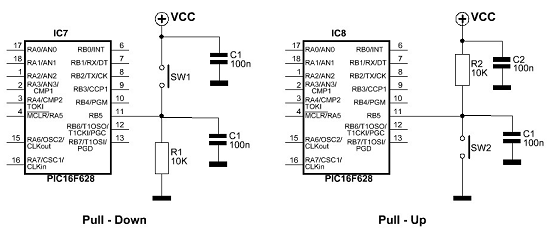
\includegraphics[width=12cm]{capitulo2/figs/fig4.png}
\caption{Condensador Bypass}
\end{figure}

\end{itemize}

Para circuitos mas complejos se deben de llevar acabo ciertas consideraciones dependiendo de los niveles de potencia a manejar. En nuestro caso 


\newpage
\section{Fuente de voltaje lineal}
Es común en proyectos de electrónica no especializados la utilización de diferentes tipos de fuentes de voltaje, entre las que se encuentran fuentes lineales, conmutadas, boost o tipo buck y los problemas que puede causar la falta de atención en este punto tan crucial puede afectan los resultados finales de un proyecto. Es por ello que se necesita conocer los principios fundamentales que reinan a este tipo de sistemas que gobernaran el comportamiento de nuestro proyecto al nivel mas básico.\\

La fuente de voltaje lineal consiste en un sistema sencillo y estructurado, el cual se diseña en diferentes configuraciones en cada modulo a partir del tipo de carga que requiere el proyecto. Para ello podemos observar en la figura 2.5 de manera ilustrativa el orden de la estructura básica de una fuente lineal.

\begin{figure}[H]
 \centering
 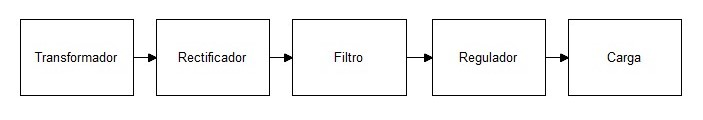
\includegraphics[width=12cm]{capitulo2/figs/fuentelineal.jpg}
 \caption{estructura fuente lineal}
 \end{figure}
 
 De manera independiente podemos analizar cada aspecto presentado en la imagen, el cual, de uno en uno se va realizando un análisis para definir los valores y topologias que satisfacen las necesidades requeridas. Tomando en cuenta lo mencionado podemos comenzar a definir las ecuaciones y modelos existentes.
\subsection{Transformador}
\subsection{Rectificador}

\subsection{Filtro}
\subsection{regulador}
\subsection{carga}


\newpage
\section{Disipadores de calor}
\section{Micro-controlador}
sda
\section{Inversores de voltaje}
\section{Bobina de ignición}
das
\section{Fuentes de alto voltaje mas comunes}


\section{Multiplicador de voltaje Cockcroft-Walton}
fgdgf